% Diagram of Android activity life cycle
% Author: Pavel Seda 
\documentclass[border=10pt]{standalone}
\usepackage{tikz}

\usetikzlibrary{arrows.meta, shapes, chains, arrows, shadows}

% Set up a few colours


\tikzset{%
  >={Latex[width=2mm,length=2mm]},
  % Specifications for style of nodes:
	base/.style = {draw, on chain, on grid, align=center, minimum height=4ex},
	Docs/.style = {base, fill=blue!30},
	screen/.style = {base, fill=orange!15},
	form/.style = {on chain, on grid, align=center, minimum height=4ex, fill=white},
    computer/.style = {base, fill=green!30},
    decision/.style={base, diamond, aspect=2.5, fill=red!30,text width=5em},
	process/.style = {base, minimum width=2.5cm, fill=orange!15,
                           font=\ttfamily},                       
    coord/.style={coordinate, on chain, on grid, node distance=6mm and 25mm},
	norm/.style={->, draw, black},  
	multidoc/.style={
		base,
		shape=tape,
		tape bend top=none,
		fill=white,
		double copy shadow,
		fill=blue!30
	},
	end/.style={
		base,
		shape=ellipse,
		fill={rgb:red,1;green,2;blue,5},
		text=white
	}
}
\begin{document}    
% Drawing part, node distance is 1.5 cm and every node
% is prefilled with white background

\resizebox{\textwidth}{!}{%
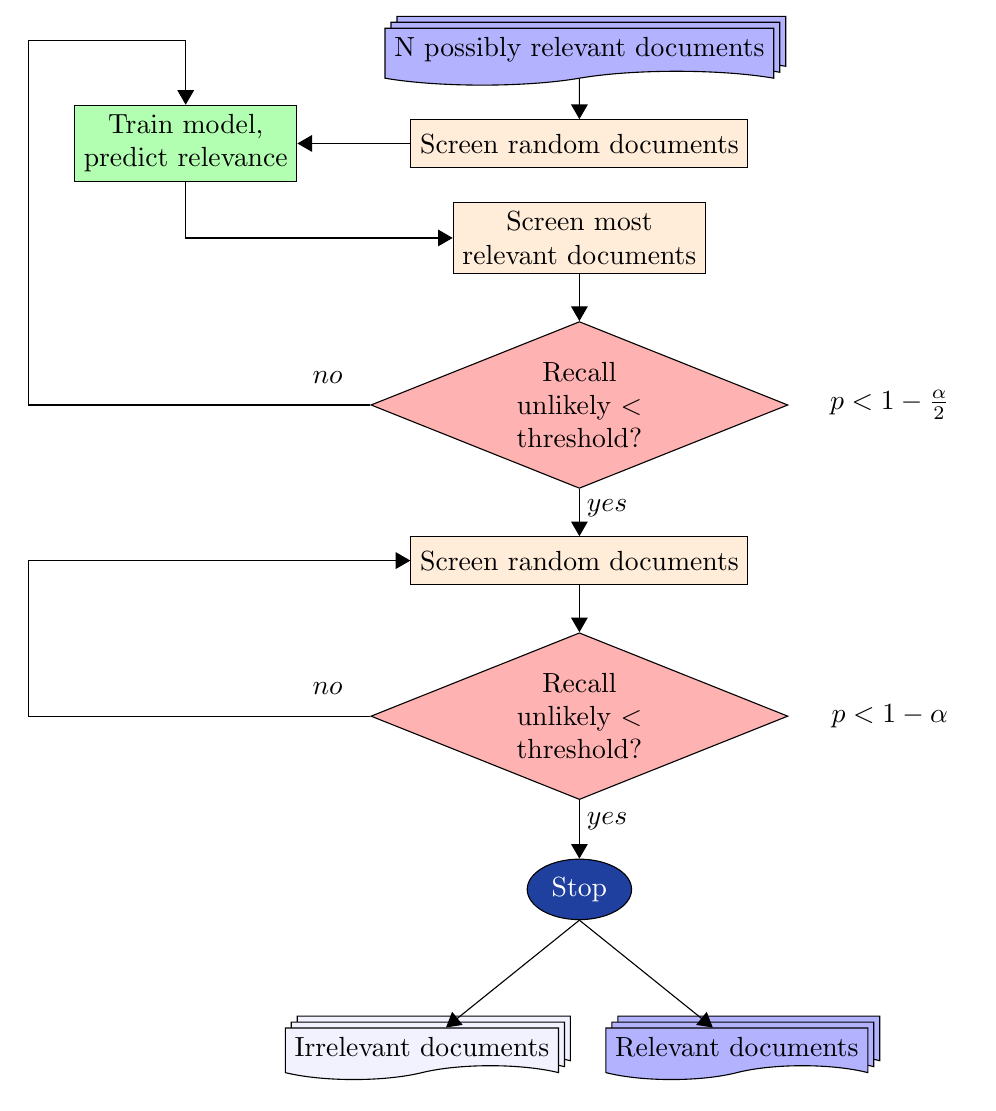
\begin{tikzpicture}[
    >=triangle 60,              % Nice arrows; your taste may be different
start chain=going below,    % General flow is top-to-bottom
node distance=6mm and 50mm, % Global setup of box spacing
every join/.style={norm},   % Default linetype for connecting boxes
]
%    every node/.style={fill=white, font=\sffamily}, align=center]
  % Specification of nodes (position, etc.)
  \node (docs)  [multidoc]  {N possibly relevant documents};
  
  \node (sample)  [screen, join]  {Screen random documents};
  \node (model) [computer, join, left=of sample]  {Train model,\\ predict relevance};
  \node (screenrel)  [screen, below of =sample]  {Screen most \\ relevant documents};
  \node (stopscreen) [decision, join] {Recall unlikely $<$ threshold?};
  
  \node (screenr2) [screen, join]  {Screen random documents};
  
  \node (recall) [decision, join] {Recall unlikely $<$ threshold?};
  
    	\node (e1) [form, right=of stopscreen, xshift=-10mm] { $p < 1-\frac{\alpha}{2}$ };
  
	%\node (sform) [form, right=of screenr2, xshift=-15mm] { Estimate $\hat{p}U$ };
  
  \node (rform) [form, right=of recall, xshift=-10mm] { $p < 1-\alpha $ };
  
  \node (stop) [end, below of=recall, yshift=-10mm] {Stop};
  
  \node (reldocs) [multidoc, below of=stop, xshift=20mm, yshift=-8mm]  {Relevant documents};
  \node (irreldocs) [multidoc, fill=blue!5, below of=stop, xshift=-20mm, yshift=-8mm]  {Irrelevant documents};
  %\node 
  
  
  \draw [o->,norm] (model.south) |-  (screenrel.west);
 
  
  \node [coord, left=of stopscreen, xshift=-45mm] (c1)  {}; %\cmark{1} 
  \node [coord, above=of model, yshift=2em] (c2)  {}; %\cmark{1} 
  
  \node [coord, left=of recall, xshift=-45mm] (c3)  {}; %\cmark{1} 
  
 \path (stopscreen.west) to node [very near start, yshift=1em] {$no$} (c1); 
 
 	\draw [o->,norm] (stopscreen.west) -- (c1) |-  (c2) -- (model.north);
 	
  \path (recall.west) to node [very near start, yshift=1em] {$no$} (c3); 
  
    \path (stopscreen.south) to node [very near start, yshift=-0.5em, xshift=1em] {$yes$} (screenr2.north); 
    
    \path (recall.south) to node [very near start, yshift=-0.5em, xshift=1em] {$yes$} (stop.north); 
 
 %\draw [o->,norm] (recall.west) -- (c3) |-  (c2) -- (model.north);
 \draw [o->,norm] (recall.west) -- (c3) |-  (screenr2.west);
 
 \draw [o->,norm] (recall.south) -- (stop);
 
 \draw [o->,norm] (stop.south) -- (reldocs);
 \draw [o->,norm] (stop.south) -- (irreldocs);
 	
 	
 	
 	
  
  \end{tikzpicture}
}
\end{document}